\documentclass[]{report}

\usepackage{graphicx}
\usepackage[svgnames]{xcolor}
\usepackage[colorlinks=true, linkcolor=Maroon, urlcolor=Maroon]{hyperref}

% Title Page
\title{Project Report - Securing Information Exchange with Blockchain}
\author{Harsh Kedia}


\begin{document}
	\maketitle

	\begin{abstract}
		Existing applications for sharing files are central solutions and therefore suffer from the single point of failure risk. Moreover, using central services for securing data means that we have to trust a 3rd party with our data thus exposing it to manipulation risks. Hence, a decentralized application was required to overcome the problems posed by a central application. With the recent developments in Blockchain technology and P2P storage, it's possible to securely store and share data without using any central service.
		
		This report outlines my master's project which is about securing information exchange using Blockchains. I describe here the workings of my application 'dShare' built using P2P technologies enabling a secure way of storing and sharing data between two individuals or entities.
		
		For storing files, I use InterPlanetary File System (IPFS), which is a P2P file storage protocol. Before uploading to the IPFS network, files are encrypted using AES-GCM encryption mechanism. Sharing of keys is facilitated using smart contracts built on Ethereum, thus files can be shared by anyone having a Ethereum address. Finally, for immutable timestamping, OriginStamp is used, which submits a file's hash to the Bitcoin blockchain.
		
		
		I implemented the front-end using React.js, a JavaScript framework. Solidity was used to write smart contracts and deployed on the Ethereum test network (Rinkeby). Next.js was used for server side rendering (SSR) and Firebase was used as a database for storing public Ethereum key of the users.
	\end{abstract}

	\section*{Project Motivation}
		Today's supply chain spans multiple geographies but the documents involved in the industry such as delivery certificates are still in physical form. This paperwork prevents manipulations but leads to various delays across the whole chain, thus affecting everyone involved.
		
		Above problem can be solved by digitizing all documents, time-stamping them using a trusted Time stamping authority (TSA) and upload them to a cloud service. However, the tools used to accomplish this solution are central services, and, therefore, suffers from data manipulations by a 3rd party.
		
		We, therefore, need a solution that is peer-to-peer (P2P) and decentralized. Blockchain offer a means of decentralized time stamping and enables peer-to-peer storage systems that are resistant to manipulations by any 3rd party.
		
		This project describes the working of an application build using decentralized technologies such as Bitcoin, Ethereum and IPFS such that it's capable of immutable timestamping and secure file sharing in a P2P manner.
	
	\section*{Related Work}
		Below is a list of related work in immutable timestamping and decentralized storage explored as part of the project.
		
		\subsection*{Proof of Existence}
			It's a web based service that implements the concept of immutable timestamping using the Bitcoin blockchain. It notarizes data in the blockchain by submitting the hash of the data in a Bitcoin transaction. Currently, the service required 0.00025BTC\footnote{\url{https://poex.io/prove}} for every certification which makes it expensive to timestamp large volumes of data.
			
		\subsection*{OriginStamp}
			OriginStamp\footnote{\url{https://originstamp.org/}} extends the concept of Proof of Existence by providing a scalable protocol which overcomes the transaction limitations of the Bitcoin blockchain.
			
			When a user submits a file, the hash of the data is recorded. Instead of creating a Bitcoin transaction for each submitted hash, it combines all the hashes submitted over a time period and generates an aggregated hash. After some additional hashing and encoding operations, a Bitcoin address is created, to which the smallest possible transactional amount of Bitcoins is transferred. Performing this transaction embeds the hash and the timestamp permanently to the Bitcoin blockchain.
			
		\subsection*{Chainpoint}
			It works similarly to OriginStamp. The service runs on the Tierion\footnote{\url{https://tierion.com/}} Network, providing a scalable protocol for anchoring data in the blockchain and generating blockchain receipts. These receipts are called chainpoint proofs which defines a path of operations that cryptographically links the data to one or more blockchains.
			
		\subsection*{Sia}
			Sia\cite{vorick2014sia} is a decentralized cloud storage system that allow its users to rent storage among peers by means of storage contracts which are cryptographically secured by saving on a blockchain. This makes the storage contracts tamper-proof and publicaly auditable.
			
			To ensure that storage provider holds a client’s data at a given time, they constantly need to submit storage proofs. The network consensus allows automatic verification of storage proofs and enforcement of storage contracts. The availability of data is ensured using redundancy techniques such as erasure codes.
			
			Sia uses a variant of Bitcoin blockchain for storing the contracts and the user must use Siacoin, an ERC-20 token in order to transact on the Sia network.
		
		\subsection*{Storj}
			Storj works similarly to Sia. It's built on Kademlia DHT, connecting peers who can transact with each other. A transaction can involve negotiation of storage contract, transfer of data, verifying remote data, download data or payments to other nodes. Each peer is capable of doing transactions independently without any human involvement.
			
			Storj uses the Ethereum blockchain for managing its storage contracts. They are stored as versioned data structure describing the relationship between a client and a storage provider. Users must use Storjcoin, an ERC-20 token to perform transactions on the Storj network. 
		
		\subsection*{InterPlanetary File System (IPFS)}
			Unlike Sia and Storj, IPFS is a P2P file transfer protocol which connects all peers in the network by a shared file system. It achieves this by combining previous peer-to-peer systems such as DHT, BitTorrent, and Git. The data in the IPFS network are modeled as a Merkle DAG thus providing a throughput storage system with content-addressed hyperlinks.
			
			To transact on the IPFS network, a user does not need any tokens.
	
	\section*{Approach}
		Below is a comparison between different timestamping methods and decentralized storage techniques explored above.
		
		\begin{figure}[h]
			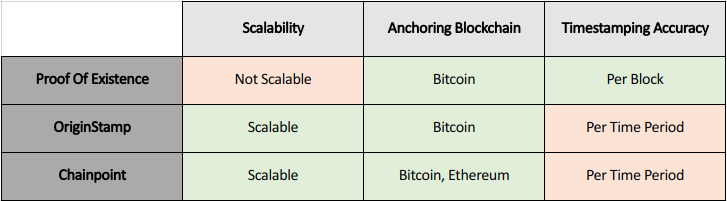
\includegraphics[width=\linewidth]{comparison-timestamping.png}
			\caption{Comparing Decentralized Timestamping}
			\label{fig:comparison-timestamping}
		\end{figure}
	
		Comparing the decentralized timestamping solutions, Proof of Existence creates a Bitcoin transaction for each hash submitted by the user. Moreover, each certification costs 0.00025 BTC. These limitations make it impractical and expensive for timestamping large volume of data. Both OriginStamp and Chainpoint, instead of creating a transaction for each submitted hash, concatenates the submitted hashes over a period and creates a single transaction with the aggregated hash. Thus they overcome the limitations of Proof of Existence and provide a scalable protocol which can handle large volumes of data.
	
		\begin{figure}[h]
			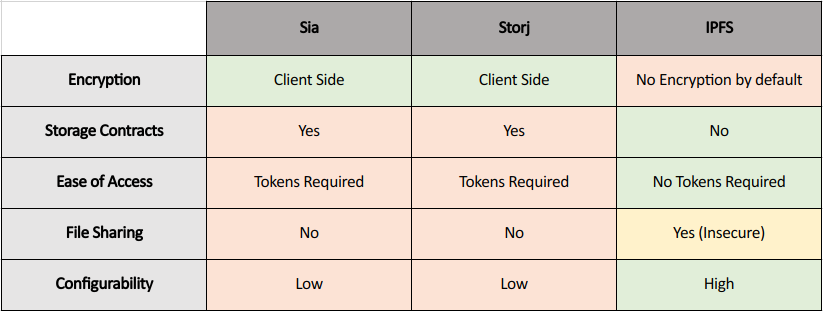
\includegraphics[width=\linewidth]{comparison-storage.png}
			\caption{Comparing Decentralized Storage}
			\label{fig:comparison-storage}
		\end{figure}
	
		Comparing the decentralized storage systems, both Sia and Storj provide an encrypted data storage; however current implementations do not allow for file sharing. Moreover, both require platform specific crypto tokens to access the network. IPFS, on the other hand, does not encrypt files by default. Files on the IPFS network are accessed by their hashes; thus anyone who knows the file’s hash can access the file. There are no storage contracts involved for storing files on the network. IPFS network does not require any crypto token for the users to access the network.
		
		Looking at the limitations of the existing solutions, we propose a solution for secure information exchange  with blockchains using smart contracts, immutable timestamping and decentralized storage.
		
		For timestamping both OriginStamp and Chainpoint can be used as they can handle large volumes of data and provide a rich set of APIs for integrating decentralized timestamping in any application. For decentralized storage, we want to use IPFS as it is a general-purpose file storage protocol and does not require any crypto tokens for access to its network and for exchanging document encryption keys, we want to use the Ethereum smart contracts.
	
	\section*{Implementation}
		
	
	\section*{Results}
	
	\section*{Future Work}
	
	\bibliographystyle{acm}
	\bibliography{report}
\end{document}          
